\documentclass[11pt]{article}
\usepackage[margin=1in]{geometry}
\usepackage{amsmath,amssymb,amsthm,mathtools}
\usepackage{graphicx}
\usepackage[hidelinks]{hyperref}
\usepackage{xcolor}
\usepackage{enumitem}

\newtheorem{theorem}{Theorem}
\newtheorem{proposition}{Proposition}
\newtheorem{remark}{Remark}
\newcommand{\R}{\mathbb{R}}
\newcommand{\N}{\mathbb{N}}
\newcommand{\ellTwo}{\ell^2}

\title{Counterexamples to Two Galerkin Projection Lemmas\\
in arXiv:1610.04776}
\author{Candidate counterexample packet for human review}
\date{27 August 2026}

\begin{document}
\maketitle

\begin{center}
\fbox{\parbox{0.91\textwidth}{
\textbf{Status.} Candidate counterexample, likely valid.  The packet refutes
Theorems 6.2 and 6.3 as stated in the source paper.  It identifies a proof gap
in the Galerkin derivation of the principal equilibrium theorems, but does not
claim that those equilibrium theorems are false and does not answer the
paper's final saturation-necessity question.}}
\end{center}

\section{Source and claims under review}

The source is M. Ali Khan and Nobusumi Sagara, ``Fatou's Lemma,
Galerkin Approximations and the Existence of Walrasian Equilibria in Infinite
Dimensions,'' arXiv:1610.04776v2 (2017) \cite{KS}.

On printed page 30, Theorem 6.2 states that if \(E\) is an ordered locally
convex Hausdorff space and \(P\) is a continuous projection of \(E\) onto a
closed vector subspace \(V\), then \(P:E\to V\) is positive.  On printed
pages 31--32, Theorem 6.3(i) states that, for any nested dense Galerkin scheme
\((V_n)\) in a separable Banach space and any continuous projections
\(P_n:E\to V_n\), every \((P_nx)\) has a subsequence converging weakly to
\(x\).  Part (ii) asserts the weak-star analogue for projections \(Q_n\) on
\(E^*\) (the displayed occurrence of \(Q_nx\) is naturally read as
\(Q_np\), as in its proof).

\begin{figure}[p]
\centering

\includegraphics[width=0.91\textwidth]{figures/open_problem_crop.png}
\caption{Printed page 30 of the source, containing Theorem 6.2 and its proof.}
\end{figure}

\begin{figure}[p]
\centering
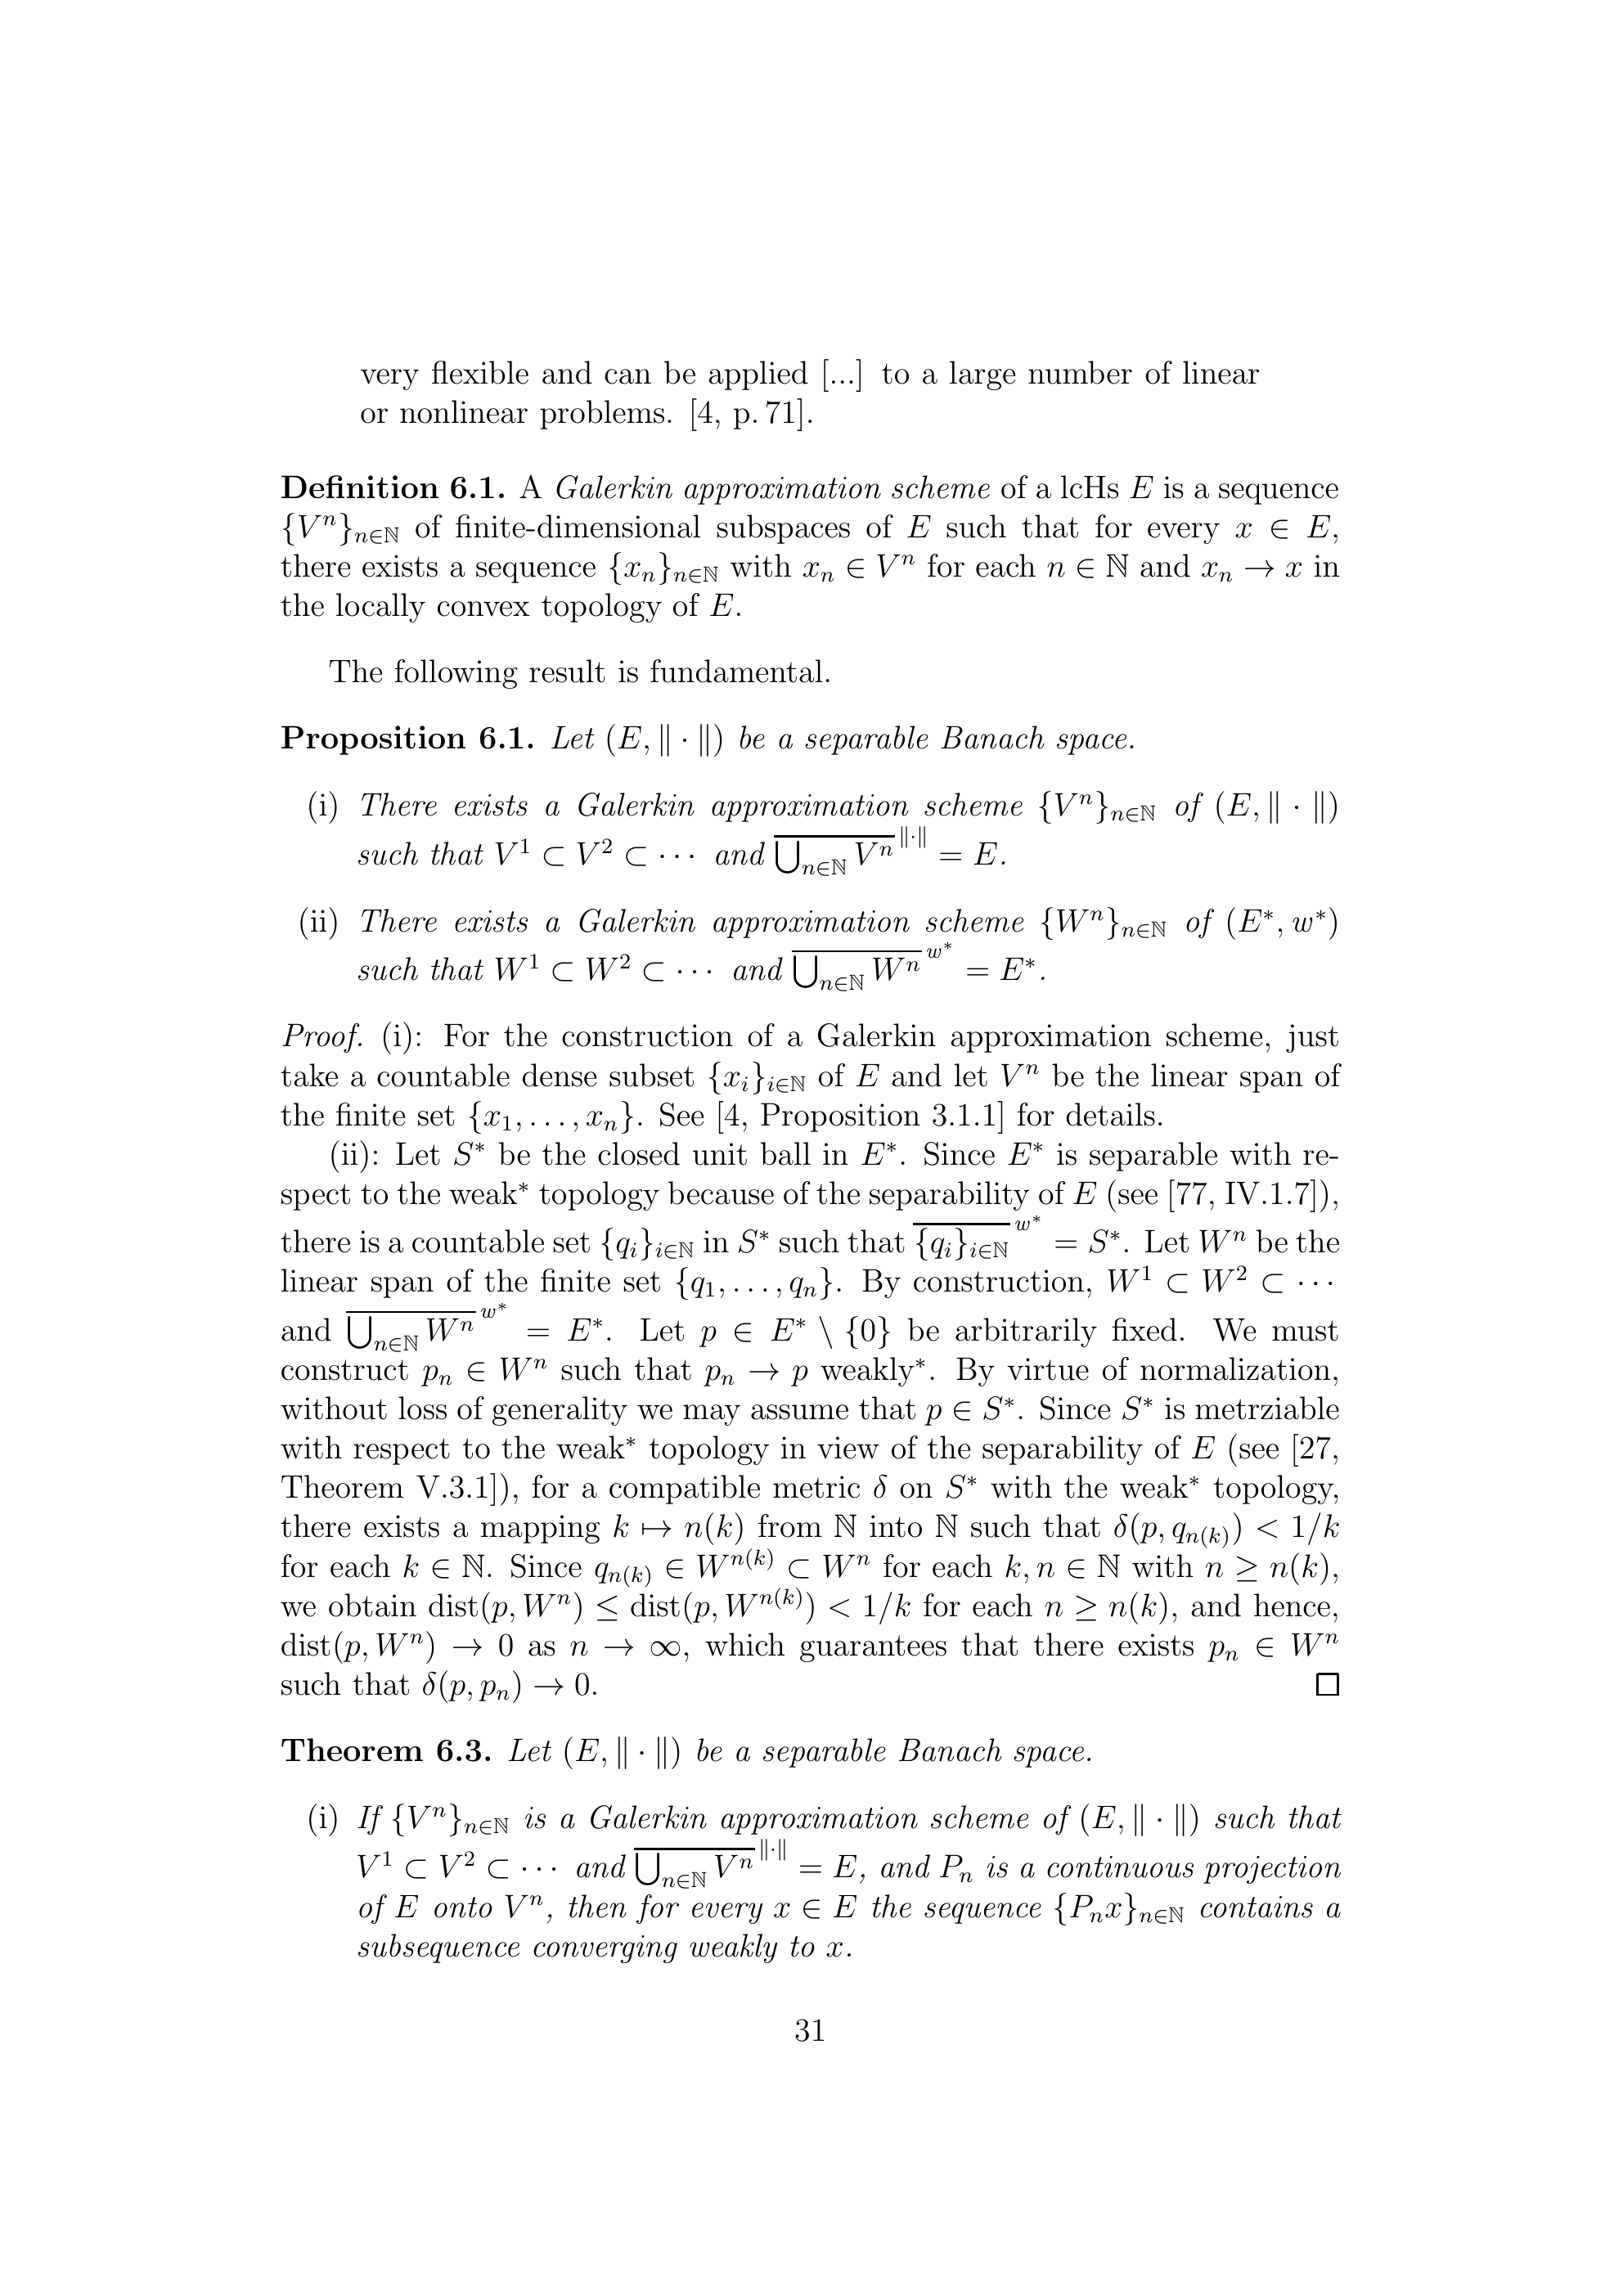
\includegraphics[width=0.91\textwidth]{figures/theorem_6_3_i.png}
\caption{Printed page 31 of the source, containing Theorem 6.3(i).}
\end{figure}

\begin{figure}[p]
\centering
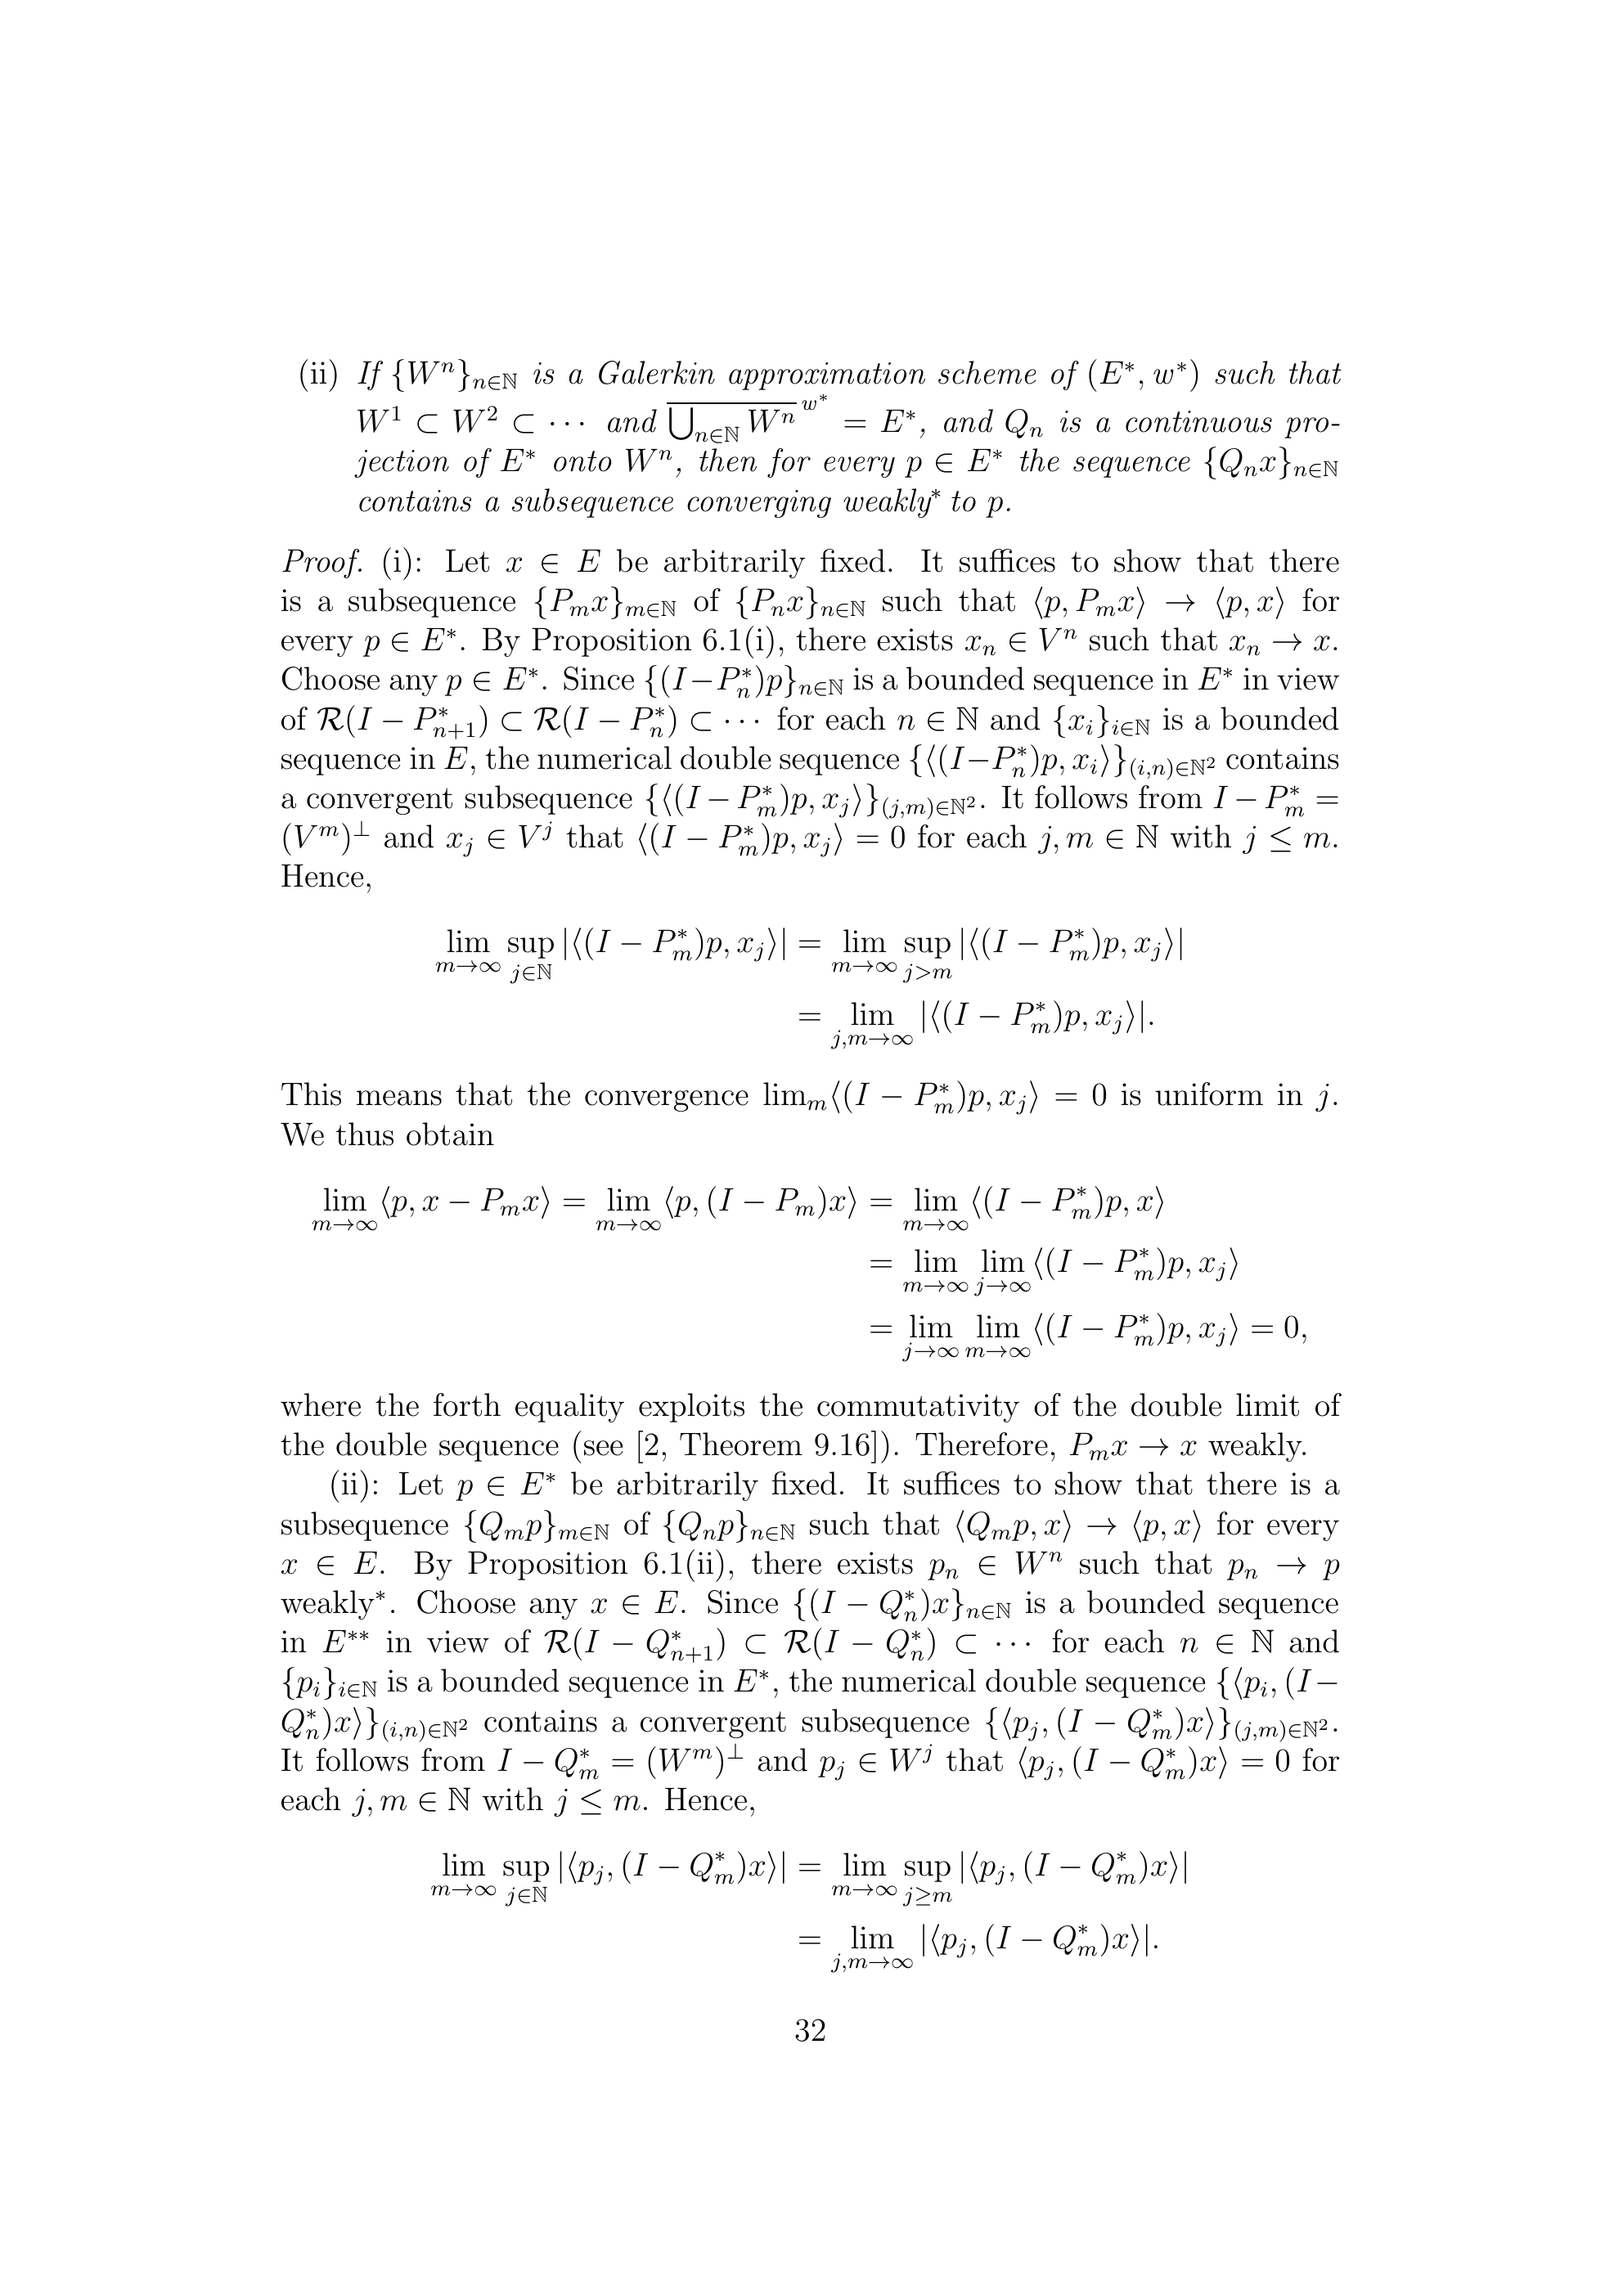
\includegraphics[width=0.91\textwidth]{figures/theorem_6_3_ii.png}
\caption{Printed page 32 of the source, containing Theorem 6.3(ii) and the
beginning of its proof.}
\end{figure}

\clearpage
\section{Idea of the proof}

Positivity is not a formal consequence of idempotence: an oblique projection
can send a positive vector outside the induced positive cone of its range.
This already happens in two dimensions.

Likewise, density of the ranges of finite-rank projections does not control
the norms of the projections.  On \(\ell^2\), start with the usual coordinate
truncation and add an increasingly large multiple of the next coordinate in
the \(e_1\)-direction.  The added term vanishes on the range, so idempotence is
preserved, while a single square-summable vector makes the first coordinate
of every projected vector diverge.  Weak convergence is then impossible.

\section{Counterexample to Theorem 6.2}

\begin{theorem}
There is an ordered finite-dimensional Banach space \(E\), a closed subspace
\(V\), and a continuous projection \(P:E\to V\) which is not positive.
Indeed, \(V\) can be chosen so that no positive projection of \(E\) onto
\(V\) exists.
\end{theorem}

\begin{proof}
Let \(E=\R^2\), with its usual norm and coordinatewise order, so
\(E_+=\R_+^2\).  Put
\[
  V=\operatorname{span}\{(1,-1)\},
  \qquad P(a,b)=(a,-a).
\]
Then \(P\) is linear and continuous, its range is \(V\), and
\[
 P^2(a,b)=P(a,-a)=(a,-a)=P(a,b),
\]
so it is a continuous projection onto the closed subspace \(V\).  However,
\((1,0)\in E_+\), whereas
\[
 P(1,0)=(1,-1)\notin E_+\cap V=V_+.
\]
Thus \(P\) is not positive.

Moreover \(V_+=V\cap E_+=\{0\}\).  If a positive projection
\(Q:E\to V\) existed, then \(Q(E_+)\subseteq V_+=\{0\}\).  Since
\(E=E_+-E_+\), linearity would force \(Q=0\), contradicting that its range
is the nonzero space \(V\).  Hence this subspace admits no positive
projection at all.
\end{proof}

There is also an immediate internal inconsistency in the printed separation
argument.  It asserts the existence of \(x^*\) such that
\(\langle Px,x^*\rangle=1\) and \(\langle y,x^*\rangle=0\) for every
\(y\in V\).  But \(Px\in V\), so the second equality applied to \(y=Px\)
already gives \(\langle Px,x^*\rangle=0\).

\section{Counterexample to Theorem 6.3}

\begin{theorem}
Both parts of Theorem 6.3 are false under their displayed hypotheses.
More precisely, there are nested finite-dimensional subspaces with dense
union and continuous projections onto them for which one fixed vector has no
subsequence of projections converging weakly to that vector.
\end{theorem}

\begin{proof}
Let \(E=\ellTwo\) with standard orthonormal basis \((e_k)_{k\ge1}\), and let
\[
  V_n=\operatorname{span}\{e_1,\ldots,e_n\}.
\]
Then \(V_1\subset V_2\subset\cdots\), and the union is norm dense in
\(\ellTwo\).  For \(x=(x_k)_{k\ge1}\), define
\[
  P_nx=\sum_{k=1}^{n}x_ke_k+n^3x_{n+1}e_1.
  \tag{1}
\]
Each \(P_n\) is bounded, since
\[
  \|P_nx\|_2
  \le \left\|\sum_{k=1}^{n}x_ke_k\right\|_2+n^3|x_{n+1}|
  \le (1+n^3)\|x\|_2.
\]
Its range is contained in \(V_n\), and if \(y\in V_n\), then
\(y_{n+1}=0\), so \(P_ny=y\).  Consequently
\(P_n^2=P_n\) and \(\mathcal R(P_n)=V_n\): it is a continuous projection
onto the required Galerkin subspace.

Now take
\[
  x_1=0,\qquad x_k=\frac1{k^2}\quad(k\ge2).
\]
This vector belongs to \(\ellTwo\).  Evaluation against \(e_1\), a
continuous linear functional on \(\ellTwo\), gives
\[
  \langle P_nx,e_1\rangle
  =x_1+n^3x_{n+1}
  =\frac{n^3}{(n+1)^2}\longrightarrow+\infty.
\]
Every subsequence has indices tending to infinity, so no subsequence of
\((P_nx)\) can converge weakly to \(x\) (or weakly to any vector).  This
refutes part (i).

For part (ii), identify \(E^*=\ellTwo\) in the usual self-dual way, set
\(W_n=V_n\), and set \(Q_n=P_n\).  Norm density implies weak-star density,
so \((W_n)\) is a Galerkin approximation scheme for \((E^*,w^*)\).  Taking
\(p=x\), the same pairing with \(e_1\in E\) diverges.  Hence no subsequence
of \((Q_np)\) converges weak-star to \(p\), refuting the intended assertion
of part (ii).
\end{proof}

\section{Where the printed proof fails and a repair}

The source proof says that \(((I-P_n^*)p)\) is bounded ``in view of'' an
inclusion of ranges.  The displayed assumptions impose neither compatibility
of the projections nor uniform boundedness of their operator norms; the
counterexample has \(\|P_n\|\ge n^3\).  Mere inclusion of finite-dimensional
ranges cannot supply the missing norm estimate.

A standard sufficient repair for part (i) is
\[
  \sup_n\|P_n\|<\infty.
  \tag{2}
\]
Indeed, write \(M=\sup_n\|P_n\|\).  Given \(x\in E\) and \(\varepsilon>0\),
choose \(m\) and \(y\in V_m\) with \(\|x-y\|<\varepsilon/(M+1)\).
For every \(n\ge m\), nestedness gives \(y\in V_n\), hence \(P_ny=y\), and
\[
 \|P_nx-x\|
 \le \|P_n(x-y)\|+\|y-x\|
 <\varepsilon.
\]
Thus (2) yields the stronger conclusion \(P_nx\to x\) in norm.  Positivity,
however, requires an independent order-theoretic hypothesis; it does not
follow from continuity and idempotence.

\section{Impact on the equilibrium arguments}

In Step 1 of the proof of Theorem 7.1, the source explicitly invokes
Theorem 6.2 to assert that \(P_n:E\to V_n\) is positive and hence that
\(P_n(X(t))\subset V_{n,+}\).  In Step 2 it invokes Theorem 6.3(i) to identify
weak limits of the projected endowments.  The proof of Theorem 7.2 repeats
the same scheme in the weak-star setting.  The counterexamples above show
that these two inputs are unavailable under the hypotheses stated in
Section 6.

There is a further definitional issue in Step 1: the source sets
\(X^n(t)=P_n(X(t))\) and calls \(\succsim_n(t)\) the restriction of a
preference relation originally defined only on \(X(t)\) to
\(X^n(t)\).  For a general projection, \(P_n(X(t))\) need not be contained in
\(X(t)\), so such a restriction need not be defined.

These observations establish a proof gap, not a counterexample to Theorems
7.1 or 7.2.  Other equilibrium-existence methods or stronger approximation
hypotheses may repair the main conclusions.  They also do not decide the
concluding question asking whether saturation is necessary.

\section{Verification and novelty check}

The proof is algebraic.  The accompanying script
\texttt{code/check\_finite\_truncations.py} checks, for finite test vectors and
many values of \(n\), that (1) is idempotent on its finite-coordinate model,
fixes \(V_n\), and has the predicted divergent first coordinate.  These
checks are sanity tests, not a substitute for the proof.

A bounded novelty search on 27 August 2026 covered: the arXiv corpus and the
run's local indexes for the paper id, title, ``continuous projection,''
``positive linear operator,'' ``Theorem 6.2,'' and ``Theorem 6.3''; web
searches for the exact theorem phrase, the title together with ``erratum'' or
``projection positive,'' and the authors together with ``Galerkin
projection.''  The search found the original arXiv record and a 2017 talk
repeating the positivity step, but no erratum or published correction.  This
is evidence only within the stated search bounds, not a claim of exhaustive
novelty.

\section{Human-review recommendation}

\begin{enumerate}[leftmargin=*]
\item Verify that the published version has the same hypotheses as arXiv
      v2, especially whether compatibility or uniform boundedness of the
      projections was added.
\item Check whether Theorems 7.1 and 7.2 have independent proofs in the cited
      equilibrium literature; the present result concerns the proof printed
      here.
\item If communicating the issue to the authors, lead with the two-line
      \(\R^2\) counterexample and the explicit \(\ell^2\) family (1).
\end{enumerate}

\begin{thebibliography}{9}
\bibitem{KS}
M. Ali Khan and N. Sagara,
\emph{Fatou's Lemma, Galerkin Approximations and the Existence of Walrasian
Equilibria in Infinite Dimensions}, Pure Appl. Funct. Anal. 2 (2017),
317--355; arXiv:1610.04776v2.
\end{thebibliography}

\end{document}
